\documentclass[a4paper,11pt]{article}
\usepackage[utf8]{inputenc}
\usepackage[T1]{fontenc}
\usepackage{amsmath,amssymb}
\usepackage[a4paper,left=2cm,right=2cm,top=3.6cm,bottom=2.3cm,headheight=1.1cm,headsep=0.6cm,footskip=1cm]{geometry}
\usepackage{xcolor}
\usepackage{tikz}
\usetikzlibrary{calc,arrows.meta,positioning,shapes.geometric,matrix}
\usepackage{fancyhdr}
\usepackage{lastpage}
\usepackage{tabularx}
\usepackage{array}
\usepackage[most]{tcolorbox}
\usepackage{enumitem}
\usepackage{needspace}

% ---------- palet sky (Sky-800 dan Sky-200) ----------
\definecolor{mainc}{HTML}{075985}
\definecolor{accc}{HTML}{0284C7}
\definecolor{skyl}{HTML}{BAE6FD}
\definecolor{deepc}{HTML}{082F49}
\definecolor{softbg}{HTML}{F0F9FF}
\definecolor{warmc}{HTML}{D97706}
\definecolor{brick}{HTML}{B91C1C}
\newcommand{\dis}{\displaystyle}

\setlength{\parindent}{0pt}
\renewcommand{\arraystretch}{1.35}

\tikzset{
  ar/.style={-{Stealth[length=1.8mm]},thick,mainc},
  box/.style={draw=mainc,thick,rounded corners=3pt,fill=softbg,align=center,inner sep=4pt},
  ax/.style={-{Stealth[length=1.6mm]},thick,mainc}
}

% ---------- header ----------
\pagestyle{fancy}
\fancyhf{}
\renewcommand{\headrulewidth}{0pt}
\fancyhead[L]{%
  \begin{tikzpicture}[remember picture,overlay]
    \fill[mainc] ([yshift=-1.2cm]current page.north west) rectangle ([yshift=-3.15cm]current page.north east);
    \fill[skyl] ([yshift=-3.15cm]current page.north west) rectangle ([yshift=-3.3cm]current page.north east);
  \end{tikzpicture}%
  \color{white}\bfseries\large Latihan Soal Irisan Kerucut}
\fancyhead[R]{\color{white}\small Diunduh dari website \textbf{Math1729}\ \,|\,\ 5 Oktober 2026}
\fancyfoot[L]{\small\color{mainc}Math1729 --- Irisan Kerucut}
\fancyfoot[R]{\small\color{mainc}Halaman \thepage\ dari \pageref{LastPage}}

% ---------- komponen ----------
\newcounter{no}
\newcommand{\bagian}[2]{\par\Needspace{6\baselineskip}\vspace{1.0em}\noindent
  \begin{tcolorbox}[colback=mainc,colframe=mainc,coltext=white,boxrule=0pt,arc=2pt,left=6pt,right=6pt,top=3pt,bottom=3pt]
  \textbf{#1}\hfill{\small #2}\end{tcolorbox}\setcounter{no}{0}\par\vspace{-0.3em}}
\newcommand{\tingkat}[2]{\par\Needspace{7\baselineskip}\vspace{0.6em}\noindent
  {\color{accc}\rule{3pt}{1.1em}}\ {\color{mainc}\bfseries #1}\ {\small\color{gray}--- #2}\par\vspace{0.1em}}
\newcommand{\soal}[2]{\par\vspace{0.75em}\stepcounter{no}\noindent
  \begin{minipage}[t]{1.8em}\textbf{\theno.}\end{minipage}%
  \begin{minipage}[t]{\dimexpr\linewidth-1.8em\relax}#1\par\vspace{0.35em}#2\end{minipage}\par}
\newcommand{\poin}[1]{\hfill{\small\color{mainc}[#1 poin]}}
\newcommand{\gbr}[2]{\noindent\begin{minipage}[t]{0.54\linewidth}#1\end{minipage}\hfill\raisebox{\ht\strutbox}{\begin{minipage}[t]{0.43\linewidth}\vspace{0pt}\centering#2\end{minipage}}}
\newcommand{\pil}[5]{\begin{tabularx}{\linewidth}{@{}*{5}{X}@{}}\textbf{A.}\;#1 & \textbf{B.}\;#2 & \textbf{C.}\;#3 & \textbf{D.}\;#4 & \textbf{E.}\;#5\end{tabularx}}
\newcommand{\pilx}[5]{\begin{tabularx}{\linewidth}{@{}*{3}{X}@{}}\textbf{A.}\;#1 & \textbf{B.}\;#2 & \textbf{C.}\;#3\\[10pt] \textbf{D.}\;#4 & \textbf{E.}\;#5 & \end{tabularx}}
\newcommand{\jwb}{\hfill Jawaban: \rule{4.5cm}{0.4pt}}
\begin{document}
\thispagestyle{fancy}

\begin{center}
  {\color{mainc}\fontsize{22}{26}\selectfont\bfseries Latihan Soal Irisan Kerucut\par}
  \vspace{2pt}
  {\color{accc}\large Lingkaran, Garis Singgung, Elips, Parabola, Hiperbola, dan Penalaran Geometri Analitik\par}
\end{center}
\vspace{2pt}
\begin{tcolorbox}[colback=softbg,colframe=mainc!40,boxrule=0.6pt,arc=3pt,left=8pt,right=8pt,top=5pt,bottom=5pt]
\noindent\textbf{Nama} : \rule{4.6cm}{0.4pt}\hfill\textbf{Kelas} : \rule{2.2cm}{0.4pt}\hfill\textbf{Skor} : \rule{2.2cm}{0.4pt}
\end{tcolorbox}
\vspace{2pt}
\begin{tcolorbox}[colback=white,colframe=accc,boxrule=0.8pt,arc=3pt,left=8pt,right=8pt,top=4pt,bottom=4pt,title={\bfseries Petunjuk Pengerjaan},coltitle=white,fonttitle=\small]
\small
\begin{enumerate}[leftmargin=1.4em,itemsep=1pt,topsep=1pt]
\item Soal terdiri atas \textbf{20 pilihan ganda} (5 mudah, 6 sedang, 7 sulit, 2 HOTS), \textbf{5 isian singkat} (2 sedang, 3 sulit), dan \textbf{5 uraian (essay)} (2 sedang, 2 sulit, 1 HOTS). Soal disusun berjenjang dan memakai bentuk yang sejalan dengan UTBK-SNBT 2026: pilihan ganda lima opsi, pilihan majemuk kompleks (menentukan benar atau salah tiap pernyataan), isian singkat, serta soal berkonteks dengan gambar atau diagram. Soal uraian ditambahkan untuk melatih penalaran tertulis. Alokasi waktu yang disarankan: 120 menit.
\item Skor: pilihan ganda 2 poin, isian singkat 4 poin, uraian 8 poin per soal (total 100 poin). Tidak ada pengurangan skor untuk jawaban salah.
\item Notasi: $e=\frac ca$ eksentrisitas; elips $c^2=a^2-b^2$; hiperbola $c^2=a^2+b^2$; $F$ fokus; $O$ titik asal $(0,0)$. Panjang latus rektum elips $\frac{2b^2}{a}$ dan parabola $4p$. Gambar tidak selalu digambar sesuai skala; bila ada kotak-kotak, satu petak menyatakan satu satuan.
\item Bilangan ribuan ditulis dengan tanda titik dan bilangan desimal dengan tanda koma. Pada isian singkat, tuliskan hanya jawaban akhir (boleh berbentuk akar atau pecahan).
\item Kalkulator tidak diperkenankan. Hasil perhitungan boleh dibiarkan dalam bentuk akar atau pecahan.
\end{enumerate}
\end{tcolorbox}

% =====================================================================
\bagian{A. Pilihan Ganda}{20 soal $\times$ 2 poin = 40 poin. Pilih satu jawaban yang paling tepat.}

\tingkat{Tingkat Mudah}{soal 1 sampai 5}
\soal{\gbr{Gambar menunjukkan sebuah lingkaran pada bidang koordinat (satu petak = satu satuan) dengan pusat $P$ dan titik $T$ yang terletak pada lingkaran. Persamaan lingkaran tersebut adalah \dots.}{%
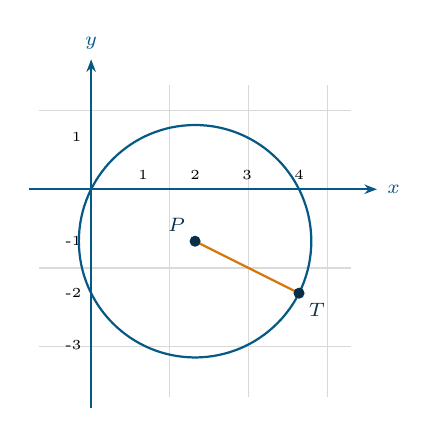
\begin{tikzpicture}[x=0.66cm,y=0.66cm]
\draw[gray!30] (-1,-4) grid (5,2);
\draw[ax] (-1.2,0)--(5.5,0) node[right,font=\scriptsize]{$x$};
\draw[ax] (0,-4.2)--(0,2.5) node[above,font=\scriptsize]{$y$};
\foreach \i in {1,2,3,4}{\node[font=\tiny,above] at (\i,0) {\i};}
\foreach \j in {-3,-2,-1,1}{\node[font=\tiny,left] at (0,\j) {\j};}
\draw[mainc,thick] (2,-1) circle ({sqrt(5)});
\draw[warmc,thick] (2,-1)--(4,-2);
\fill[deepc] (2,-1) circle (2pt) node[above left,font=\scriptsize\bfseries]{$P$};
\fill[deepc] (4,-2) circle (2pt) node[below right,font=\scriptsize\bfseries]{$T$};
\end{tikzpicture}}}{\pilx{$(x+2)^2+(y-1)^2=5$}{$(x-2)^2+(y+1)^2=25$}{$(x-2)^2+(y+1)^2=5$}{$(x-4)^2+(y+2)^2=5$}{$(x-2)^2+(y+1)^2=3$}}
\soal{Koordinat fokus elips $16x^2+25y^2=400$ adalah \dots.}{\pil{$(\pm3,0)$}{$(\pm\sqrt{41},0)$}{$(0,\pm3)$}{$(\pm4,0)$}{$(\pm5,0)$}}
\soal{Fokus dan persamaan direktriks parabola $x^2=-8y$ berturut-turut adalah \dots.}{\pilx{$(0,2)$ dan $y=-2$}{$(0,-2)$ dan $y=2$}{$(-2,0)$ dan $x=2$}{$(0,-4)$ dan $y=4$}{$(0,-8)$ dan $y=8$}}
\soal{Persamaan asimtot hiperbola $9x^2-16y^2=144$ adalah \dots.}{\pil{$y=\pm\frac43x$}{$y=\pm\frac{16}9x$}{$y=\pm\frac9{16}x$}{$y=\pm\frac34x$}{$y=\pm\frac54x$}}
\soal{Tentukan nilai kebenaran tiga pernyataan berikut (B = benar, S = salah), berurutan dari (i) sampai (iii).\par\smallskip
(i) Persamaan $2x^2+2y^2-8=0$ menyatakan sebuah elips.\par
(ii) Persamaan $x^2+4y^2-4=0$ menyatakan sebuah elips.\par
(iii) Persamaan $y^2-4x+2y+9=0$ menyatakan sebuah parabola.}{\pilx{B, B, B}{B, S, B}{S, S, B}{B, B, S}{S, B, B}}

\tingkat{Tingkat Sedang}{soal 6 sampai 11}
\soal{Garis $g$ menyinggung lingkaran $x^2+y^2-4x+6y-12=0$ di titik $(6,0)$. Luas daerah segitiga yang dibatasi oleh garis $g$ dan kedua sumbu koordinat adalah \dots\ satuan luas.}{\pil{$24$}{$12$}{$32$}{$48$}{$36$}}
\soal{Garis $4x+3y=k$ menyinggung lingkaran $x^2+y^2+2x-4y-4=0$. Jumlah semua nilai $k$ yang mungkin adalah \dots.}{\pil{$2$}{$4$}{$13$}{$17$}{$30$}}
\soal{Luas persegi panjang terkecil yang sisi-sisinya sejajar sumbu koordinat dan memuat seluruh elips $4x^2+9y^2-16x+18y-11=0$ adalah \dots\ satuan luas.}{\pil{$12$}{$18$}{$20$}{$24$}{$36$}}
\soal{Titik $P(x,y)$ bergerak sehingga jaraknya ke titik $F(3,2)$ selalu sama dengan jaraknya ke garis $x=-1$. Persamaan lintasan titik $P$ adalah \dots.}{\pilx{$(y-2)^2=4(x-1)$}{$(y-2)^2=8(x+1)$}{$(y-2)^2=8(x-1)$}{$(x-1)^2=8(y-2)$}{$(y-2)^2=16(x-1)$}}
\soal{Titik $P$ bergerak sehingga selisih mutlak jaraknya ke $A(-5,0)$ dan $B(5,0)$ selalu sama dengan $6$. Persamaan lintasan titik $P$ adalah \dots.}{\pilx{$\dfrac{x^2}{16}-\dfrac{y^2}9=1$}{$\dfrac{x^2}9+\dfrac{y^2}{16}=1$}{$\dfrac{x^2}{25}-\dfrac{y^2}9=1$}{$\dfrac{y^2}9-\dfrac{x^2}{16}=1$}{$\dfrac{x^2}9-\dfrac{y^2}{16}=1$}}
\soal{\gbr{Lingkaran $L_1:x^2+y^2-4x-6y-12=0$ dan $L_2:x^2+y^2-20x-6y+100=0$ digambar seperti di samping. Ruas garis $ST$ adalah garis singgung persekutuan luar kedua lingkaran, dengan $S$ pada $L_1$ dan $T$ pada $L_2$. Panjang ruas $ST$ adalah \dots.}{%
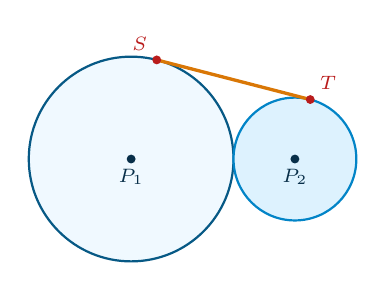
\begin{tikzpicture}[x=0.26cm,y=0.26cm]
\draw[mainc,thick,fill=softbg] (2,3) circle (5);
\draw[accc,thick,fill=skyl!50] (10,3) circle (3);
\fill[deepc] (2,3) circle (1.6pt) node[below,font=\scriptsize]{$P_1$};
\fill[deepc] (10,3) circle (1.6pt) node[below,font=\scriptsize]{$P_2$};
\coordinate (S) at (3.25,7.8412); \coordinate (T) at (10.75,5.9047);
\draw[warmc,very thick] (S)--(T);
\fill[brick] (S) circle (1.6pt) node[above left,font=\scriptsize\bfseries]{$S$};
\fill[brick] (T) circle (1.6pt) node[above right,font=\scriptsize\bfseries]{$T$};
\end{tikzpicture}}}{\pil{$4\sqrt3$}{$2\sqrt{15}$}{$2\sqrt{17}$}{$8$}{$6$}}

\tingkat{Tingkat Sulit}{soal 12 sampai 18, setara UTBK}
\soal{Lingkaran $x^2+y^2=25$ dan lingkaran $x^2+y^2-8x-6y=0$ berpotongan di dua titik. Panjang tali busur persekutuan kedua lingkaran tersebut adalah \dots.}{\pil{$5$}{$5\sqrt2$}{$8$}{$5\sqrt3$}{$10$}}
\soal{\gbr{Dari titik $Q(13,7)$ ditarik dua garis singgung ke lingkaran $x^2+y^2-2x-4y-20=0$ dengan titik singgung $A$ dan $B$ (lihat gambar). Panjang tali busur $AB$ adalah \dots.}{%
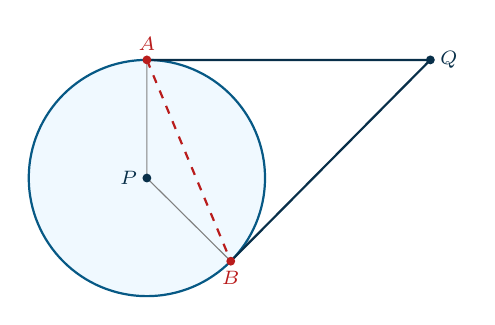
\begin{tikzpicture}[x=0.3cm,y=0.3cm]
\draw[mainc,thick,fill=softbg] (1,2) circle (5);
\coordinate (P) at (1,2); \coordinate (Q) at (13,7);
\coordinate (A) at (1,7); \coordinate (B) at (4.5503,-1.5207);
\draw[deepc,thick] (Q)--(A) (Q)--(B);
\draw[brick,dashed,thick] (A)--(B);
\draw[gray] (P)--(A) (P)--(B);
\fill[deepc] (P) circle (1.6pt) node[left,font=\scriptsize]{$P$};
\fill[deepc] (Q) circle (1.6pt) node[right,font=\scriptsize]{$Q$};
\fill[brick] (A) circle (1.6pt) node[above,font=\scriptsize]{$A$};
\fill[brick] (B) circle (1.6pt) node[below,font=\scriptsize]{$B$};
\end{tikzpicture}}}{\pil{$\dfrac{120}{13}$}{$\dfrac{60}{13}$}{$10$}{$12$}{$\dfrac{240}{13}$}}
\soal{\gbr{Elips $\dfrac{x^2}{36}+\dfrac{y^2}{16}=1$ memiliki fokus $F_1$ dan $F_2$. Titik $P$ terletak pada elips sehingga $\angle F_1PF_2=90^\circ$ (lihat gambar). Luas segitiga $F_1PF_2$ adalah \dots\ satuan luas.}{%
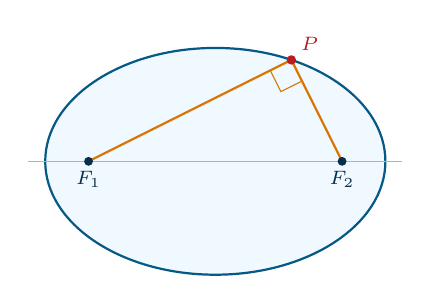
\begin{tikzpicture}[x=0.36cm,y=0.36cm]
\draw[mainc,thick,fill=softbg] (0,0) ellipse (6 and 4);
\draw[gray!60] (-6.6,0)--(6.6,0);
\coordinate (F1) at (-4.4721,0); \coordinate (F2) at (4.4721,0); \coordinate (P) at (2.6833,3.5777);
\draw[warmc,thick] (F1)--(P)--(F2);
\coordinate (m1) at ($(P)!0.3cm!(F1)$); \coordinate (m2) at ($(P)!0.3cm!(F2)$);
\coordinate (m3) at ($(m1)+(m2)-(P)$);
\draw[warmc] (m1)--(m3)--(m2);
\fill[deepc] (F1) circle (1.6pt) node[below,font=\scriptsize]{$F_1$};
\fill[deepc] (F2) circle (1.6pt) node[below,font=\scriptsize]{$F_2$};
\fill[brick] (P) circle (1.7pt) node[above right,font=\scriptsize\bfseries]{$P$};
\end{tikzpicture}}}{\pil{$12$}{$14$}{$16$}{$20$}{$24$}}
\soal{\gbr{Garis yang melalui fokus parabola $y^2=8x$ dengan gradien $1$ memotong parabola di titik $A$ dan $B$ (lihat gambar). Panjang ruas $AB$ adalah \dots.}{%
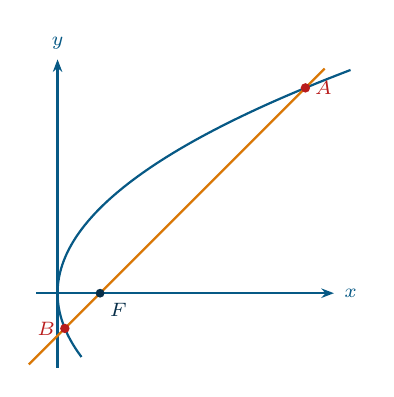
\begin{tikzpicture}[x=0.27cm,y=0.27cm]
\draw[ax] (-1,0)--(13,0) node[right,font=\scriptsize]{$x$};
\draw[ax] (0,-3.5)--(0,11) node[above,font=\scriptsize]{$y$};
\draw[mainc,thick,domain=-3:10.5,samples=60,smooth,variable=\t] plot ({\t*\t/8},{\t});
\coordinate (A) at (11.657,9.657); \coordinate (B) at (0.343,-1.657); \coordinate (F) at (2,0);
\draw[warmc,thick] ($(B)!-0.15!(A)$)--($(B)!1.08!(A)$);
\fill[deepc] (F) circle (1.6pt) node[below right,font=\scriptsize]{$F$};
\fill[brick] (A) circle (1.7pt) node[right,font=\scriptsize\bfseries]{$A$};
\fill[brick] (B) circle (1.7pt) node[left,font=\scriptsize\bfseries]{$B$};
\end{tikzpicture}}}{\pil{$8$}{$10$}{$12$}{$14$}{$16$}}
\soal{Terdapat dua garis singgung hiperbola $\dfrac{x^2}{25}-\dfrac{y^2}{16}=1$ yang tegak lurus garis $3x+4y=7$. Jarak antara kedua garis singgung tersebut adalah \dots.}{\pil{$\dfrac{16}{5}$}{$\dfrac{32}{5}$}{$\dfrac{16}{3}$}{$\dfrac{32}{3}$}{$8$}}
\soal{Banyak bilangan bulat $k$ sehingga persamaan $\dfrac{x^2}{9-k}+\dfrac{y^2}{k-1}=1$ menyatakan sebuah \textbf{elips} (bukan lingkaran) adalah \dots.}{\pil{$3$}{$4$}{$5$}{$6$}{$7$}}
\soal{\gbr{Sebuah terowongan satu arah dengan penampang berbentuk setengah elips memiliki lebar dasar $12$ m dan tinggi maksimum $4$ m. Sebuah truk berpenampang persegi panjang selebar $4$ m melintas dengan sisi kirinya berjarak $1$ m dari sumbu simetri terowongan (lihat gambar). Tinggi truk maksimum agar dapat melintas adalah \dots\ m.}{%
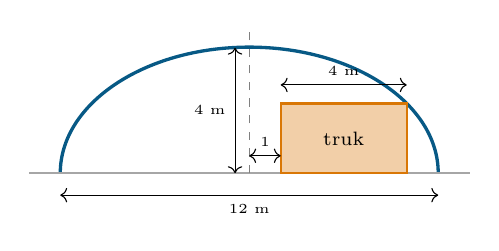
\begin{tikzpicture}[x=0.4cm,y=0.4cm]
\draw[mainc,very thick] (-6,0) arc (180:0:6 and 4);
\draw[gray!70,thick] (-7,0)--(7,0);
\draw[gray,dashed] (0,0)--(0,4.6);
\fill[warmc!35,draw=warmc,thick] (1,0) rectangle (5,2.2111);
\node[font=\scriptsize] at (3,1.1) {truk};
\draw[<->,font=\tiny] (-6,-0.7)--(6,-0.7) node[midway,below]{$12$ m};
\draw[<->] (1,2.8)--(5,2.8) node[midway,above,font=\tiny]{$4$ m};
\draw[<->] (0,0.55)--(1,0.55) node[midway,above,font=\tiny]{$1$};
\draw[<->] (-0.45,0)--(-0.45,3.98) node[midway,left,font=\tiny]{$4$ m};
\end{tikzpicture}}}{\pilx{$\dfrac23\sqrt{11}$}{$\dfrac52$}{$\dfrac43\sqrt5$}{$3$}{$4$}}

\tingkat{Tingkat HOTS}{soal 19 dan 20, penalaran tingkat tinggi gaya UTBK}
\soal{Diberikan keluarga kurva $\Gamma_\lambda:\ \dfrac{x^2}{25-\lambda}+\dfrac{y^2}{9-\lambda}=1$, dengan $\lambda$ bilangan real, $\lambda\neq9$ dan $\lambda\neq25$. Tentukan nilai kebenaran empat pernyataan berikut (B = benar, S = salah), berurutan dari (i) sampai (iv).\par\smallskip
(i) Untuk $\lambda=0$, $\Gamma_\lambda$ adalah elips dengan fokus $(\pm4,0)$.\par
(ii) Untuk $\lambda=16$, $\Gamma_\lambda$ adalah hiperbola dengan fokus $(\pm4,0)$.\par
(iii) Semua elips dalam keluarga ini memiliki eksentrisitas yang sama.\par
(iv) Tidak ada nilai $\lambda$ yang membuat $\Gamma_\lambda$ berupa lingkaran.}{\pilx{B, B, B, B}{B, S, S, B}{B, B, S, B}{S, B, S, S}{B, B, S, S}}
\soal{\gbr{Sebuah cermin berbentuk parabola $y^2=8x$ memantulkan sinar laser. Sinar dari sumber $S(18,8)$ bergerak sejajar sumbu-$x$ ke kiri, mengenai cermin di $A$, dipantulkan melalui fokus $F$, mengenai cermin lagi di $B$, lalu dipantulkan dan akhirnya mengenai layar tegak pada garis $x=18$ di titik $C$ (lihat gambar). Panjang seluruh lintasan sinar $S\to A\to B\to C$ adalah \dots.\par\smallskip\footnotesize (Petunjuk: sifat pemantulan parabola dan definisi parabola.)}{%
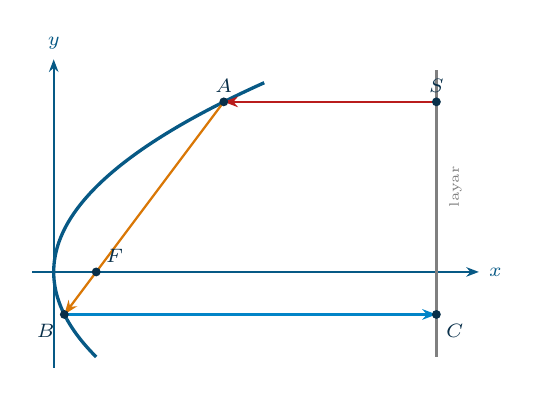
\begin{tikzpicture}[x=0.27cm,y=0.27cm]
\draw[ax] (-1,0)--(20,0) node[right,font=\scriptsize]{$x$};
\draw[ax] (0,-4.5)--(0,10) node[above,font=\scriptsize]{$y$};
\draw[mainc,very thick,domain=-4:8.9,samples=60,smooth,variable=\t] plot ({\t*\t/8},{\t});
\draw[gray,very thick] (18,-4)--(18,9.5);
\node[font=\tiny,gray,rotate=90] at (18.9,4) {layar};
\coordinate (S) at (18,8); \coordinate (A) at (8,8); \coordinate (F) at (2,0);
\coordinate (B) at (0.5,-2); \coordinate (C) at (18,-2);
\draw[ar,brick] (S)--(A);
\draw[ar,warmc] (A)--(B);
\draw[ar,accc] (B)--(C);
\fill[deepc] (F) circle (1.6pt) node[above right,font=\scriptsize]{$F$};
\fill[deepc] (S) circle (1.6pt) node[above,font=\scriptsize]{$S$};
\fill[deepc] (A) circle (1.6pt) node[above,font=\scriptsize]{$A$};
\fill[deepc] (B) circle (1.6pt) node[below left,font=\scriptsize]{$B$};
\fill[deepc] (C) circle (1.6pt) node[below right,font=\scriptsize]{$C$};
\end{tikzpicture}}}{\pil{$30$}{$32$}{$35$}{$38$}{$40$}}

% =====================================================================
\bagian{B. Isian Singkat}{5 soal $\times$ 4 poin = 20 poin. Tuliskan hanya jawaban akhir.}

\tingkat{Tingkat Sedang}{soal 1 dan 2}
\soal{Titik $P$ bergerak sehingga jaraknya ke $A(-3,0)$ selalu dua kali jaraknya ke $B(3,0)$. Lintasan titik $P$ berbentuk lingkaran dengan jari-jari \dots.}{\jwb}
\soal{Jumlah koordinat fokus parabola $y=\dfrac18x^2-x+3$ adalah \dots.}{\jwb}

\tingkat{Tingkat Sulit}{soal 3 sampai 5}
\soal{Titik $P$ bergerak pada elips $\dfrac{x^2}{16}+\dfrac{y^2}{9}=1$ dengan fokus $F_1$ dan $F_2$. Luas maksimum segitiga $PF_1F_2$ adalah \dots.}{\jwb}
\soal{\gbr{Hiperbola $\dfrac{x^2}9-\dfrac{y^2}{16}=1$ berfokus di $F_1$ dan $F_2$. Titik $P$ pada hiperbola memenuhi $PF_1:PF_2=3:1$ (lihat gambar). Luas segitiga $PF_1F_2$ adalah \dots.}{%
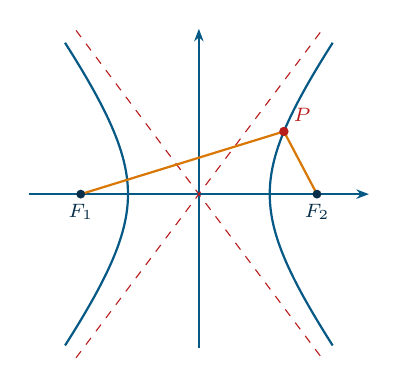
\begin{tikzpicture}[x=0.3cm,y=0.3cm]
\draw[ax] (-7.2,0)--(7.2,0); \draw[ax] (0,-6.5)--(0,7);
\draw[brick,dashed] (-5.2,-6.93)--(5.2,6.93) (-5.2,6.93)--(5.2,-6.93);
\draw[mainc,thick,domain=-1.25:1.25,samples=40,smooth,variable=\t] plot ({3*cosh(\t)},{4*sinh(\t)});
\draw[mainc,thick,domain=-1.25:1.25,samples=40,smooth,variable=\t] plot ({-3*cosh(\t)},{4*sinh(\t)});
\coordinate (F1) at (-5,0); \coordinate (F2) at (5,0); \coordinate (P) at (3.6,2.6533);
\draw[warmc,thick] (F1)--(P)--(F2);
\fill[deepc] (F1) circle (1.6pt) node[below,font=\scriptsize]{$F_1$};
\fill[deepc] (F2) circle (1.6pt) node[below,font=\scriptsize]{$F_2$};
\fill[brick] (P) circle (1.7pt) node[above right,font=\scriptsize\bfseries]{$P$};
\end{tikzpicture}}}{\jwb}
\soal{Sebuah lingkaran berpusat di fokus parabola $x^2=8y$ dan menyinggung direktriks parabola tersebut. Jarak antara kedua titik potong lingkaran dan parabola adalah \dots.}{\jwb}

% =====================================================================
\Needspace{16\baselineskip}
\bagian{C. Uraian (Essay)}{5 soal $\times$ 8 poin = 40 poin. Tuliskan langkah penyelesaian dengan lengkap.}

\tingkat{Tingkat Sedang}{soal 1 dan 2}
\soal{\gbr{Diberikan lingkaran $L:\ x^2+y^2+2x-8y-8=0$ dan titik $A(2,0)$, $B(5,8)$ seperti pada gambar.\par\smallskip
(a) Tentukan pusat dan jari-jari $L$.\par
(b) Tentukan kedudukan titik $A$ dan titik $B$ terhadap $L$.\par
(c) Tentukan persamaan garis singgung $L$ di titik $A$.\par
(d) Tentukan persamaan garis singgung $L$ lainnya yang sejajar dengan garis pada (c), lalu hitung jarak kedua garis singgung tersebut dan jelaskan hasilnya.}{%
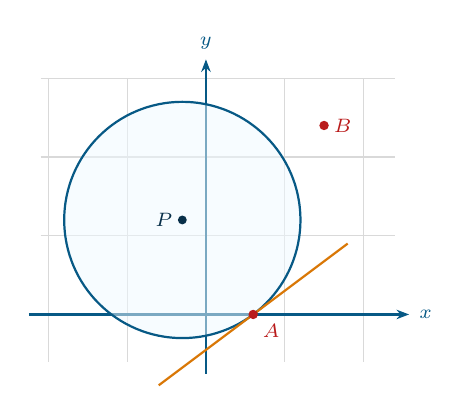
\begin{tikzpicture}[x=0.3cm,y=0.3cm]
\draw[gray!30] (-7,-2) grid (8,10);
\draw[ax] (-7.5,0)--(8.6,0) node[right,font=\scriptsize]{$x$};
\draw[ax] (0,-2.5)--(0,10.8) node[above,font=\scriptsize]{$y$};
\draw[mainc,thick,fill=softbg,fill opacity=0.5] (-1,4) circle (5);
\draw[warmc,thick] (-2,-3)--(6,3);
\fill[deepc] (-1,4) circle (1.6pt) node[left,font=\scriptsize]{$P$};
\fill[brick] (2,0) circle (1.7pt) node[below right,font=\scriptsize\bfseries]{$A$};
\fill[brick] (5,8) circle (1.7pt) node[right,font=\scriptsize\bfseries]{$B$};
\end{tikzpicture}}}{\poin{8}}
\soal{\gbr{Sebuah komet mengelilingi Matahari dengan lintasan berbentuk elips, dan Matahari berada di salah satu fokus. Jarak terdekat komet ke Matahari adalah $4$ satuan astronomi (SA) dan jarak terjauhnya $16$ SA (lihat gambar). Pusat lintasan berada di titik asal dan sumbu mayornya terletak pada sumbu-$x$.\par\smallskip
(a) Tentukan panjang setengah sumbu mayor $a$, jarak fokus $c$, dan setengah sumbu minor $b$.\par
(b) Tentukan persamaan lintasan komet.\par
(c) Tentukan eksentrisitas lintasan, lalu hitung jarak komet ke Matahari saat komet berada di ujung sumbu minor. Jelaskan mengapa hasilnya sama dengan $a$.\par
(d) Tentukan jarak komet ke Matahari saat komet berada tepat di atas Matahari (satu garis tegak lurus sumbu mayor).}{%
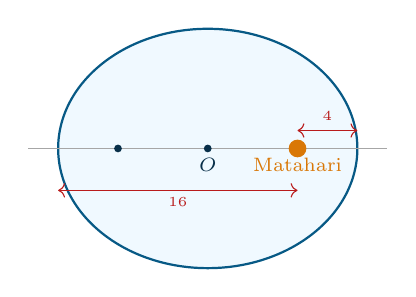
\begin{tikzpicture}[x=0.19cm,y=0.19cm]
\draw[mainc,thick,fill=softbg] (0,0) ellipse (10 and 8);
\draw[gray!70] (-12,0)--(12,0);
\coordinate (M) at (6,0);
\fill[warmc] (M) circle (3.2pt) node[below,font=\scriptsize]{Matahari};
\fill[deepc] (-6,0) circle (1.4pt);
\fill[deepc] (0,0) circle (1.4pt) node[below,font=\scriptsize]{$O$};
\draw[<->,brick] (6,1.2)--(10,1.2) node[midway,above,font=\tiny]{$4$};
\draw[<->,brick] (6,-2.8)--(-10,-2.8) node[midway,below=-1pt,font=\tiny]{$16$};
\end{tikzpicture}}}{\poin{8}}

\Needspace{22\baselineskip}
\tingkat{Tingkat Sulit}{soal 3 dan 4}
\soal{\gbr{Diberikan parabola $y^2=12x$ dengan fokus $F$ (lihat gambar).\par\smallskip
(a) Tentukan koordinat fokus, persamaan direktriks, dan panjang latus rektum.\par
(b) Garis $y=x+k$ menyinggung parabola. Tentukan nilai $k$ dan titik singgung $T$.\par
(c) Garis singgung pada (b) memotong sumbu-$x$ di titik $Q$. Tentukan koordinat $Q$.\par
(d) Buktikan bahwa $FT=FQ$, dan buktikan bahwa kaki garis tegak lurus dari $F$ ke garis singgung terletak pada sumbu-$y$. Apa makna $FT=FQ$ pada pemantulan sinar dari $F$?}{%
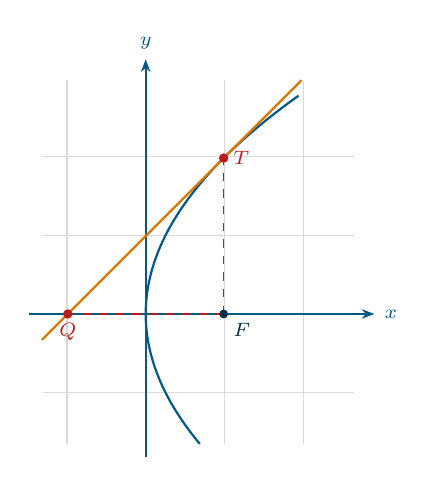
\begin{tikzpicture}[x=0.33cm,y=0.33cm]
\draw[gray!30] (-4,-5) grid (8,9);
\draw[ax] (-4.5,0)--(8.8,0) node[right,font=\scriptsize]{$x$};
\draw[ax] (0,-5.5)--(0,9.8) node[above,font=\scriptsize]{$y$};
\draw[mainc,thick,domain=-5:8.4,samples=60,smooth,variable=\t] plot ({\t*\t/12},{\t});
\draw[warmc,thick] (-4,-1)--(6,9);
\coordinate (F) at (3,0); \coordinate (T) at (3,6); \coordinate (Q) at (-3,0);
\draw[brick,dashed] (F)--(T) (F)--(Q);
\fill[deepc] (F) circle (1.6pt) node[below right,font=\scriptsize]{$F$};
\fill[brick] (T) circle (1.7pt) node[right,font=\scriptsize\bfseries]{$T$};
\fill[brick] (Q) circle (1.7pt) node[below,font=\scriptsize\bfseries]{$Q$};
\end{tikzpicture}}}{\poin{8}}
\soal{\gbr{Dua stasiun radio $A$ dan $B$ berada di pantai lurus pada koordinat $A(-50,0)$ dan $B(50,0)$ (satuan km). Sebuah kapal $P$ menerima sinyal dari kedua stasiun pada saat yang sama dan menghitung bahwa selisih jaraknya ke kedua stasiun selalu $60$ km, yaitu $|PA-PB|=60$ (lihat gambar).\par\smallskip
(a) Tentukan persamaan lintasan kapal.\par
(b) Jika kapal berada di titik $P$ dengan absis $60$ dan ordinat positif, tentukan koordinat $P$, lalu hitung $PA$ dan $PB$.\par
(c) Tentukan persamaan asimtot lintasan kapal.\par
(d) Sebuah perahu bergerak lurus sepanjang garis $4x-3y=20$. Tentukan titik potong garis tersebut dengan lintasan kapal, dan jelaskan mengapa hanya ada satu titik potong.}{%
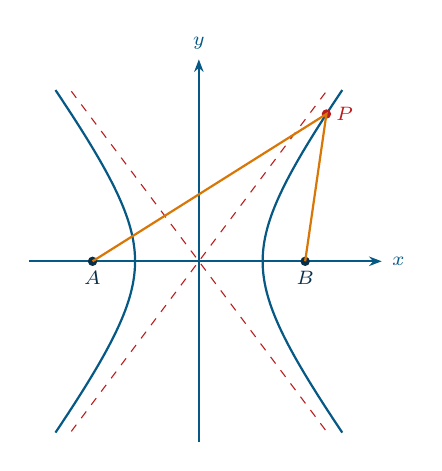
\begin{tikzpicture}[x=0.27cm,y=0.27cm]
\draw[ax] (-8,0)--(8.6,0) node[right,font=\scriptsize]{$x$};
\draw[ax] (0,-8.5)--(0,9.5) node[above,font=\scriptsize]{$y$};
\draw[brick,dashed] (-6,-8)--(6,8) (-6,8)--(6,-8);
\draw[mainc,thick,domain=-1.45:1.45,samples=40,smooth,variable=\t] plot ({3*cosh(\t)},{4*sinh(\t)});
\draw[mainc,thick,domain=-1.45:1.45,samples=40,smooth,variable=\t] plot ({-3*cosh(\t)},{4*sinh(\t)});
\fill[deepc] (-5,0) circle (1.7pt) node[below,font=\scriptsize\bfseries]{$A$};
\fill[deepc] (5,0) circle (1.7pt) node[below,font=\scriptsize\bfseries]{$B$};
\fill[brick] (6,6.928) circle (1.7pt) node[right,font=\scriptsize\bfseries]{$P$};
\draw[warmc,thick] (-5,0)--(6,6.928)--(5,0);
\end{tikzpicture}}}{\poin{8}}

\Needspace{26\baselineskip}
\tingkat{Tingkat HOTS}{soal 5}
\soal{\gbr{Diberikan lingkaran $\Gamma:\ x^2+y^2=25$ dan elips $E:\ \dfrac{x^2}{25}+\dfrac{y^2}{9}=1$. Untuk setiap titik $P(x_0,y_0)$ pada $\Gamma$, garis tegak melalui $P$ memotong $E$ di titik $Q$ yang berabsis sama dengan $P$ dan berada di sisi sumbu-$x$ yang sama dengan $P$ (lihat gambar).\par\smallskip
(a) Tunjukkan bahwa $Q\left(x_0,\tfrac35y_0\right)$.\par
(b) Untuk $x_0\neq0$, buktikan bahwa garis singgung $\Gamma$ di $P$ dan garis singgung $E$ di $Q$ berpotongan di sebuah titik pada sumbu-$x$ yang sama.\par
(c) Panjang setiap tali busur vertikal $E$ adalah $\tfrac35$ kali panjang tali busur vertikal $\Gamma$ pada absis yang sama. Dengan fakta ini, jelaskan mengapa luas daerah $E$ sama dengan $\tfrac35$ luas daerah $\Gamma$, lalu hitung luas daerah $E$.\par
(d) Untuk $P(3,4)$, tentukan $Q$, persamaan kedua garis singgung, dan titik potongnya.}{%
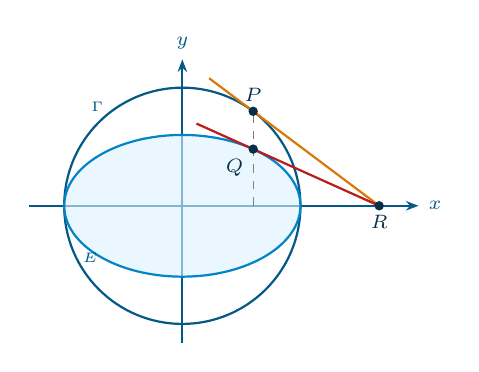
\begin{tikzpicture}[x=0.3cm,y=0.3cm]
\draw[ax] (-6.5,0)--(10,0) node[right,font=\scriptsize]{$x$};
\draw[ax] (0,-5.8)--(0,6.2) node[above,font=\scriptsize]{$y$};
\draw[mainc,thick] (0,0) circle (5);
\draw[accc,thick,fill=skyl!50,fill opacity=0.6] (0,0) ellipse (5 and 3);
\coordinate (P) at (3,4); \coordinate (Q) at (3,2.4); \coordinate (R) at (8.3333,0);
\draw[gray,dashed] (3,0)--(P);
\draw[warmc,thick] (R)--($(R)!1.35!(P)$);
\draw[brick,thick] (R)--($(R)!1.45!(Q)$);
\fill[deepc] (P) circle (1.7pt) node[above,font=\scriptsize\bfseries]{$P$};
\fill[deepc] (Q) circle (1.7pt) node[below left,font=\scriptsize\bfseries]{$Q$};
\fill[deepc] (R) circle (1.7pt) node[below,font=\scriptsize\bfseries]{$R$};
\node[font=\tiny,mainc] at (-3.6,4.2) {$\Gamma$};
\node[font=\tiny,accc!70!black] at (-3.9,-2.2) {$E$};
\end{tikzpicture}}}{\poin{8}}

% =====================================================================
\newpage
\bagian{Kunci Jawaban dan Pembahasan Singkat}{Untuk guru dan pembahasan mandiri}
\par\vspace{0.6em}{\bfseries\color{mainc}Kunci Pilihan Ganda}\par\vspace{0.3em}
\small
\begin{tabularx}{\linewidth}{@{}*{10}{>{\centering\arraybackslash}X}@{}}\hline \textbf{1} & \textbf{2} & \textbf{3} & \textbf{4} & \textbf{5} & \textbf{6} & \textbf{7} & \textbf{8} & \textbf{9} & \textbf{10}\\ \hline C & A & B & D & E & A & B & D & C & E\\ \hline\end{tabularx}\\[6pt]
\begin{tabularx}{\linewidth}{@{}*{10}{>{\centering\arraybackslash}X}@{}}\hline \textbf{11} & \textbf{12} & \textbf{13} & \textbf{14} & \textbf{15} & \textbf{16} & \textbf{17} & \textbf{18} & \textbf{19} & \textbf{20}\\ \hline B & D & A & C & E & B & D & A & C & E\\ \hline\end{tabularx}
\par\vspace{0.4em}{\bfseries\color{mainc}Kunci Isian Singkat:}\ \ 1) $4$\quad 2) $7$\quad 3) $3\sqrt7$\quad 4) $4\sqrt{11}$\quad 5) $8$
\par\vspace{0.8em}{\bfseries\color{mainc}\normalsize Pembahasan Pilihan Ganda}\par\vspace{0.2em}
\small\begin{enumerate}[leftmargin=2em,itemsep=2pt,topsep=2pt]
\item[\textbf{1.}] \textbf{(C)} Pusat $P(2,-1)$. Jari-jari adalah jarak $PT$: $r^2=(4-2)^2+(-2+1)^2=5$. Persamaannya $(x-2)^2+(y+1)^2=5$. (Jebakan: menulis $r=5$ padahal yang bernilai $5$ adalah $r^2$, atau terbalik tanda pusat.)
\item[\textbf{2.}] \textbf{(A)} Bagi dengan $400$: $\frac{x^2}{25}+\frac{y^2}{16}=1$, sehingga $a^2=25$, $b^2=16$, $c^2=a^2-b^2=9$, $c=3$. Sumbu mayor horizontal, fokus $(\pm3,0)$. (Jebakan: memakai $c^2=a^2+b^2$ sehingga diperoleh $\sqrt{41}$.)
\item[\textbf{3.}] \textbf{(B)} $x^2=-8y$ berarti $4p=8$, $p=2$, parabola terbuka ke bawah. Fokus $(0,-p)=(0,-2)$ dan direktriks $y=p=2$.
\item[\textbf{4.}] \textbf{(D)} $9x^2-16y^2=144\Rightarrow\frac{x^2}{16}-\frac{y^2}{9}=1$, jadi $a=4$, $b=3$. Asimtot $y=\pm\frac bax=\pm\frac34x$. (Nilai $\frac54$ adalah eksentrisitas $\frac ca$, bukan gradien asimtot.)
\item[\textbf{5.}] \textbf{(E)} (i) $2x^2+2y^2=8\Rightarrow x^2+y^2=4$ adalah \emph{lingkaran} (koefisien $x^2$ dan $y^2$ sama), jadi \textbf{S}. (ii) $x^2+4y^2=4\Rightarrow\frac{x^2}4+y^2=1$ adalah elips, \textbf{B}. (iii) $(y+1)^2=4x-8=4(x-2)$ adalah parabola, \textbf{B}. Urutan: S, B, B.
\item[\textbf{6.}] \textbf{(A)} Lingkaran: $(x-2)^2+(y+3)^2=25$. Titik $(6,0)$ terletak pada lingkaran karena $16+9=25$. Garis singgung: $(6-2)(x-2)+(0+3)(y+3)=25\Rightarrow4x+3y=24$. Titik potong sumbu: $(6,0)$ dan $(0,8)$. Luas $\frac12\cdot6\cdot8=24$.
\item[\textbf{7.}] \textbf{(B)} Pusat $(-1,2)$ dan $r^2=1+4+4=9$, $r=3$. Syarat menyinggung: jarak pusat ke garis $4x+3y-k=0$ sama dengan $r$: $\frac{|4(-1)+3(2)-k|}{5}=\frac{|2-k|}5=3\Rightarrow k=17$ atau $k=-13$. Jumlahnya $4$. (Jebakan: hanya mengambil satu nilai, atau menjumlahkan harga mutlak.)
\item[\textbf{8.}] \textbf{(D)} $4(x^2-4x)+9(y^2+2y)=11\Rightarrow4(x-2)^2+9(y+1)^2=36\Rightarrow\frac{(x-2)^2}9+\frac{(y+1)^2}4=1$. Jadi $a=3$, $b=2$. Persegi panjang terkecil menyinggung elips di empat puncaknya, dengan panjang $2a=6$ dan lebar $2b=4$. Luas $24$.
\item[\textbf{9.}] \textbf{(C)} Dari $PF=PL$: $(x-3)^2+(y-2)^2=(x+1)^2$. Maka $(y-2)^2=(x+1)^2-(x-3)^2=8x-8=8(x-1)$. Cek: puncak di tengah antara fokus dan direktriks, yaitu $(1,2)$, dengan $p=2$.
\item[\textbf{10.}] \textbf{(E)} Selisih jarak tetap menunjukkan hiperbola dengan $2a=6$, sehingga $a=3$. Fokus $(\pm5,0)$ memberi $c=5$ dan $b^2=c^2-a^2=16$. Persamaannya $\frac{x^2}9-\frac{y^2}{16}=1$.
\item[\textbf{11.}] \textbf{(B)} $L_1$: pusat $(2,3)$, $r_1=5$. $L_2$: $(x-10)^2+(y-3)^2=9$, pusat $(10,3)$, $r_2=3$. Jarak pusat $d=8=r_1+r_2$, jadi bersinggungan di luar. Panjang garis singgung persekutuan luar $=\sqrt{d^2-(r_1-r_2)^2}=\sqrt{64-4}=\sqrt{60}=2\sqrt{15}$. (Cek: untuk lingkaran bersinggungan luar, panjangnya $2\sqrt{r_1r_2}=2\sqrt{15}$.)
\item[\textbf{12.}] \textbf{(D)} Kurangkan kedua persamaan: $8x+6y-25=0$ (garis kuasa, memuat tali busur persekutuan). Jarak $O$ ke garis: $\frac{25}{\sqrt{64+36}}=\frac52$. Panjang tali busur $=2\sqrt{25-\left(\frac52\right)^2}=2\sqrt{\frac{75}4}=5\sqrt3$. (Cek: dua lingkaran berjari-jari $5$ dengan jarak pusat $5$ membentuk segitiga sama sisi.)
\item[\textbf{13.}] \textbf{(A)} Lingkaran: $(x-1)^2+(y-2)^2=25$, pusat $P(1,2)$, $r=5$. $PQ=\sqrt{12^2+5^2}=13$, sehingga garis singgung $QA=\sqrt{13^2-5^2}=12$. $AB$ tegak lurus $PQ$ dan membelah di tengah; tinggi segitiga siku-siku $PAQ$ dari $A$ ke $PQ$ adalah $\frac{PA\cdot QA}{PQ}=\frac{60}{13}$. Jadi $AB=2\cdot\frac{60}{13}=\frac{120}{13}$. (Jebakan: $\frac{60}{13}$ hanya setengah tali busur.)
\item[\textbf{14.}] \textbf{(C)} $a=6$, $b=4$, $c=\sqrt{36-16}=2\sqrt5$. $PF_1+PF_2=2a=12$. Sudut siku di $P$ memberi $PF_1^2+PF_2^2=(2c)^2=80$. Maka $2\,PF_1\!\cdot\!PF_2=12^2-80=64$, $PF_1\!\cdot\!PF_2=32$. Luas $=\frac12\cdot32=16$ (sama dengan $b^2$).
\item[\textbf{15.}] \textbf{(E)} $4p=8$, $p=2$, $F(2,0)$. Garis $y=x-2$: $(x-2)^2=8x\Rightarrow x^2-12x+4=0$, jadi $x_1+x_2=12$. Karena melalui fokus, $AB=AF+BF=(x_1+p)+(x_2+p)=12+4=16$. (Cek: $\frac{4p}{\sin^2\theta}=\frac{8}{1/2}=16$.)
\item[\textbf{16.}] \textbf{(B)} Gradien garis $3x+4y=7$ adalah $-\frac34$, sehingga gradien singgung $m=\frac43$. Rumus: $y=mx\pm\sqrt{a^2m^2-b^2}=\frac43x\pm\sqrt{25\cdot\frac{16}9-16}=\frac43x\pm\frac{16}3$, yaitu $4x-3y\pm16=0$. Jarak dua garis sejajar: $\frac{|16-(-16)|}{\sqrt{16+9}}=\frac{32}5$.
\item[\textbf{17.}] \textbf{(D)} Bentuk $\frac{x^2}A+\frac{y^2}B=1$ adalah elips jika $A>0$, $B>0$, dan $A\ne B$. $9-k>0\Rightarrow k<9$ dan $k-1>0\Rightarrow k>1$, jadi $k\in\{2,3,\dots,8\}$ ($7$ nilai). $A=B$ saat $9-k=k-1$, yaitu $k=5$ (lingkaran) yang harus dikeluarkan. Jadi $6$ nilai.
\item[\textbf{18.}] \textbf{(A)} Letakkan pusat pada tengah dasar: $\frac{x^2}{36}+\frac{y^2}{16}=1$, $y\ge0$. Truk menempati $1\le x\le5$. Elips makin rendah menjauhi sumbu simetri, sehingga sudut atas truk di $x=5$ menentukan tinggi maksimum: $y=4\sqrt{1-\frac{25}{36}}=\frac{4\sqrt{11}}6=\frac23\sqrt{11}\approx2{,}21$ m. (Jebakan: memakai $x=4$ sehingga $\frac43\sqrt5\approx2{,}98$ m.)
\item[\textbf{19.}] \textbf{(C)} (i) $\lambda=0$: $\frac{x^2}{25}+\frac{y^2}9=1$, $c^2=25-9=16$, fokus $(\pm4,0)$: \textbf{B}. (ii) $\lambda=16$: $\frac{x^2}9-\frac{y^2}7=1$, $c^2=9+7=16$, fokus $(\pm4,0)$: \textbf{B}. (iii) Untuk elips ($\lambda<9$), $a^2-b^2=(25-\lambda)-(9-\lambda)=16$ selalu tetap, jadi fokusnya sama, tetapi $a$ berubah sehingga $e=\frac4{\sqrt{25-\lambda}}$ berubah (misalnya $\lambda=0$ memberi $\frac45$ dan $\lambda=-11$ memberi $\frac23$): \textbf{S}. (iv) Lingkaran menuntut $25-\lambda=9-\lambda$, mustahil: \textbf{B}. Urutan: B, B, S, B. (Keluarga ini disebut kurva-kurva sefokus.)
\item[\textbf{20.}] \textbf{(E)} $y^2=8x$: $p=2$, $F(2,0)$, direktriks $x=-2$. Sinar $y=8$ mengenai cermin di $A(8,8)$. Pantulan melalui $F$ bergradien $\frac{8}{6}=\frac43$: $y=\frac43(x-2)$. Substitusi ke $y^2=8x$: $2x^2-17x+8=0$, $x=8$ (titik $A$) atau $x=\frac12$, jadi $B\left(\frac12,-2\right)$. Di $B$ sinar dipantulkan sejajar sumbu-$x$ (ke kanan) menyusuri $y=-2$ hingga $C(18,-2)$. $SA=10$, $AB=AF+FB=(8+2)+\left(\frac12+2\right)=\frac{25}2$, $BC=\frac{35}2$. Total $10+\frac{25}2+\frac{35}2=40$. Cara cepat: $SA+AF$ sama dengan jarak $S$ ke direktriks ($20$), dan $FB+BC$ sama dengan jarak $C$ ke direktriks ($20$), jadi total $40$.
\end{enumerate}
\par\Needspace{6\baselineskip}\vspace{0.6em}{\bfseries\color{mainc}\normalsize Pembahasan Isian Singkat}\par\vspace{0.2em}
\small\begin{enumerate}[leftmargin=2em,itemsep=2pt,topsep=2pt]
\item[\textbf{1.}] \textbf{Jawaban: $4$.} $PA=2PB\Rightarrow PA^2=4PB^2$: $(x+3)^2+y^2=4\left[(x-3)^2+y^2\right]\Rightarrow3x^2+3y^2-30x+27=0\Rightarrow x^2+y^2-10x+9=0$, yaitu $(x-5)^2+y^2=16$. Jari-jari $4$ (lingkaran Apollonius).
\item[\textbf{2.}] \textbf{Jawaban: $7$.} $y=\frac18(x^2-8x)+3=\frac18(x-4)^2+1$, sehingga $(x-4)^2=8(y-1)$. Puncak $(4,1)$, $4p=8$, $p=2$, terbuka ke atas, fokus $(4,3)$. Jumlah koordinat $4+3=7$.
\item[\textbf{3.}] \textbf{Jawaban: $3\sqrt7$.} $c^2=16-9=7$, jadi $F_1F_2=2\sqrt7$ tetap sebagai alas. Tinggi segitiga adalah $|y_P|$ yang maksimum $b=3$ (di ujung sumbu minor). Luas maksimum $\frac12\cdot2\sqrt7\cdot3=3\sqrt7$.
\item[\textbf{4.}] \textbf{Jawaban: $4\sqrt{11}$.} $a=3$, $b=4$, $c=5$, sehingga $F_1F_2=10$. Pada hiperbola, $|PF_1-PF_2|=2a=6$. Dengan $PF_1=3PF_2$ diperoleh $2PF_2=6$, $PF_2=3$, $PF_1=9$. Rumus Heron dengan sisi $9,3,10$: $s=11$, luas $=\sqrt{11\cdot2\cdot8\cdot1}=\sqrt{176}=4\sqrt{11}$.
\item[\textbf{5.}] \textbf{Jawaban: $8$.} Fokus $(0,2)$ dan direktriks $y=-2$, jarak keduanya $4$, jadi jari-jari lingkaran $4$: $x^2+(y-2)^2=16$. Substitusi $x^2=8y$: $y^2+4y-12=0$, $y=2$ (nilai $y=-6$ ditolak karena $y\ge0$). Maka $x=\pm4$ dan jaraknya $8$ (sama dengan panjang latus rektum $4p$).
\end{enumerate}
\par\Needspace{8\baselineskip}\vspace{0.6em}{\bfseries\color{mainc}\normalsize Pembahasan dan Pedoman Penskoran Uraian}\par\vspace{0.2em}
\small\begin{enumerate}[leftmargin=2em,itemsep=3pt,topsep=2pt]
\item[\textbf{1.}] (a) $A=2$, $B=-8$, $C=-8$: pusat $\left(-\frac A2,-\frac B2\right)=(-1,4)$, $r=\sqrt{1+16+8}=5$. (b) $K=(x+1)^2+(y-4)^2-25$. Titik $A$: $9+16-25=0$, jadi $A$ pada lingkaran. Titik $B$: $36+16-25=27>0$, jadi $B$ di luar lingkaran. (c) $(2+1)(x+1)+(0-4)(y-4)=25\Rightarrow3x-4y=6$. (d) Garis sejajar berbentuk $3x-4y+c=0$ dengan jarak ke pusat sama dengan $r$: $\frac{|3(-1)-4(4)+c|}5=\frac{|c-19|}5=5\Rightarrow c=44$ atau $c=-6$. Nilai $c=-6$ adalah garis pada (c), maka garis lainnya $3x-4y+44=0$. Jaraknya $\frac{|44-(-6)|}5=10=2r$: kedua garis menyinggung di ujung-ujung sebuah diameter, dan jarak dua garis singgung sejajar selalu sama dengan diameter. \\ \textit{Penskoran: tiap bagian 2 poin.}
\item[\textbf{2.}] (a) Jarak terdekat $a-c=4$ dan terjauh $a+c=16$ (ujung-ujung sumbu mayor). Jumlahkan: $a=10$; kurangkan: $c=6$; $b^2=a^2-c^2=64$, $b=8$. (b) $\frac{x^2}{100}+\frac{y^2}{64}=1$. (c) $e=\frac ca=\frac35$. Titik ujung sumbu minor $(0,\pm8)$ berjarak ke fokus $(6,0)$ sebesar $\sqrt{36+64}=10=a$. Alasannya: titik itu berjarak sama ke kedua fokus, dan jumlah kedua jarak adalah $2a$, sehingga masing-masing $a$. (d) Saat di atas Matahari, $x=6$: $\frac{36}{100}+\frac{y^2}{64}=1\Rightarrow y^2=\frac{1024}{16}$, $y=\frac{32}5=6{,}4$ SA, yaitu setengah latus rektum $\frac{b^2}a$. \\ \textit{Penskoran: (a) 2 poin; (b) 2 poin; (c) 2 poin; (d) 2 poin.}
\item[\textbf{3.}] (a) $4p=12$, $p=3$: fokus $F(3,0)$, direktriks $x=-3$, latus rektum $4p=12$. (b) Substitusi $y=x+k$: $(x+k)^2=12x\Rightarrow x^2+(2k-12)x+k^2=0$. Menyinggung bila $D=0$: $(2k-12)^2-4k^2=144-48k=0\Rightarrow k=3$. Persamaan menjadi $x^2-6x+9=0$, $x=3$, $y=6$, jadi $T(3,6)$. (c) Garis $y=x+3$ memotong sumbu-$x$ di $x=-3$: $Q(-3,0)$. (d) $FT=\sqrt{0^2+6^2}=6$ dan $FQ=3-(-3)=6$, jadi $FT=FQ$ (segitiga $FTQ$ sama kaki). Kaki garis tegak lurus dari $F(3,0)$ ke $x-y+3=0$: $H=F-\frac{3-0+3}{2}(1,-1)=(3,0)-3(1,-1)=(0,3)$, terletak pada sumbu-$y$. Makna: pada segitiga sama kaki $FTQ$, garis singgung membagi sama besar sudut antara $TF$ dan arah sejajar sumbu, sehingga sinar dari $F$ yang mengenai $T$ dipantulkan sejajar sumbu parabola. \\ \textit{Penskoran: (a) 1 poin; (b) 3 poin; (c) 1 poin; (d) 3 poin.}
\item[\textbf{4.}] (a) Selisih jarak tetap $2a=60$, jadi $a=30$; fokus $c=50$; $b^2=c^2-a^2=2500-900=1600$. Persamaan: $\frac{x^2}{900}-\frac{y^2}{1600}=1$. (b) $x=60$: $\frac{3600}{900}=4$, sehingga $\frac{y^2}{1600}=3$, $y=40\sqrt3$ ($\approx69{,}3$). $P(60,40\sqrt3)$. $PA=\sqrt{110^2+4800}=\sqrt{16900}=130$ dan $PB=\sqrt{10^2+4800}=\sqrt{4900}=70$. Selisihnya $60$ (sesuai). (c) $y=\pm\frac bax=\pm\frac43x$. (d) Dari $4x-3y=20$, $y=\frac{4x-20}3$. Persamaan hiperbola dikali $14400$: $16x^2-9y^2=14400$. Substitusi: $16x^2-(4x-20)^2=14400\Rightarrow160x-400=14400\Rightarrow x=92{,}5$ dan $y=\frac{350}3$. Hanya satu titik potong karena garis $4x-3y=20$ sejajar asimtot $y=\frac43x$ (gradien sama), sehingga suku $x^2$ saling meniadakan dan persamaannya menjadi linear. \\ \textit{Penskoran: (a) 2 poin; (b) 2 poin; (c) 1 poin; (d) 3 poin.}
\item[\textbf{5.}] (a) $P$ pada $\Gamma$: $x_0^2+y_0^2=25$. Titik $\left(x_0,\frac35y_0\right)$ memenuhi $\frac{x_0^2}{25}+\frac{(3y_0/5)^2}{9}=\frac{x_0^2}{25}+\frac{y_0^2}{25}=1$, sehingga terletak pada $E$; karena absisnya sama dan sisinya sama, titik itu adalah $Q$. (b) Singgung $\Gamma$ di $P$: $x_0x+y_0y=25$. Singgung $E$ di $Q$: $\frac{x_0x}{25}+\frac{(3y_0/5)y}{9}=1$, yaitu $\frac{x_0x}{25}+\frac{y_0y}{15}=1$. Pada $y=0$ kedua garis memberi $x=\frac{25}{x_0}$, jadi keduanya berpotongan di titik $\left(\frac{25}{x_0},0\right)$ pada sumbu-$x$. (c) Luas daerah dapat dipandang sebagai jumlah irisan vertikal tipis. Setiap irisan $E$ lebarnya $\frac35$ kali irisan $\Gamma$ pada absis yang sama, jadi luas $E=\frac35\cdot\pi\cdot5^2=15\pi$ (sesuai $\pi ab=\pi\cdot5\cdot3$). (d) $Q=\left(3,\frac{12}5\right)$. Singgung $\Gamma$: $3x+4y=25$. Singgung $E$: $\frac{3x}{25}+\frac{(12/5)y}{9}=1\Rightarrow\frac{3x}{25}+\frac{4y}{15}=1\Rightarrow9x+20y=75$. Keduanya memotong sumbu-$x$ di $\left(\frac{25}3,0\right)=R$, sesuai (b). \\ \textit{Penskoran: (a) 1 poin; (b) 3 poin; (c) 2 poin; (d) 2 poin.}
\end{enumerate}
\end{document}
